% Options for packages loaded elsewhere
\PassOptionsToPackage{unicode}{hyperref}
\PassOptionsToPackage{hyphens}{url}
%
\documentclass[
  11pt,
  ignorenonframetext,
]{beamer}
\usepackage{pgfpages}
\setbeamertemplate{caption}[numbered]
\setbeamertemplate{caption label separator}{: }
\setbeamercolor{caption name}{fg=normal text.fg}
\beamertemplatenavigationsymbolsempty
% Prevent slide breaks in the middle of a paragraph
\widowpenalties 1 10000
\raggedbottom
\setbeamertemplate{part page}{
  \centering
  \begin{beamercolorbox}[sep=16pt,center]{part title}
    \usebeamerfont{part title}\insertpart\par
  \end{beamercolorbox}
}
\setbeamertemplate{section page}{
  \centering
  \begin{beamercolorbox}[sep=12pt,center]{part title}
    \usebeamerfont{section title}\insertsection\par
  \end{beamercolorbox}
}
\setbeamertemplate{subsection page}{
  \centering
  \begin{beamercolorbox}[sep=8pt,center]{part title}
    \usebeamerfont{subsection title}\insertsubsection\par
  \end{beamercolorbox}
}
\AtBeginPart{
  \frame{\partpage}
}
\AtBeginSection{
  \ifbibliography
  \else
    \frame{\sectionpage}
  \fi
}
\AtBeginSubsection{
  \frame{\subsectionpage}
}
\usepackage{amsmath,amssymb}
\usepackage{lmodern}
\usepackage{ifxetex,ifluatex}
\ifnum 0\ifxetex 1\fi\ifluatex 1\fi=0 % if pdftex
  \usepackage[T1]{fontenc}
  \usepackage[utf8]{inputenc}
  \usepackage{textcomp} % provide euro and other symbols
\else % if luatex or xetex
  \usepackage{unicode-math}
  \defaultfontfeatures{Scale=MatchLowercase}
  \defaultfontfeatures[\rmfamily]{Ligatures=TeX,Scale=1}
\fi
% Use upquote if available, for straight quotes in verbatim environments
\IfFileExists{upquote.sty}{\usepackage{upquote}}{}
\IfFileExists{microtype.sty}{% use microtype if available
  \usepackage[]{microtype}
  \UseMicrotypeSet[protrusion]{basicmath} % disable protrusion for tt fonts
}{}
\makeatletter
\@ifundefined{KOMAClassName}{% if non-KOMA class
  \IfFileExists{parskip.sty}{%
    \usepackage{parskip}
  }{% else
    \setlength{\parindent}{0pt}
    \setlength{\parskip}{6pt plus 2pt minus 1pt}}
}{% if KOMA class
  \KOMAoptions{parskip=half}}
\makeatother
\usepackage{xcolor}
\IfFileExists{xurl.sty}{\usepackage{xurl}}{} % add URL line breaks if available
\IfFileExists{bookmark.sty}{\usepackage{bookmark}}{\usepackage{hyperref}}
\hypersetup{
  pdftitle={Nodes and Claims},
  pdfauthor={Macartan Humphreys},
  hidelinks,
  pdfcreator={LaTeX via pandoc}}
\urlstyle{same} % disable monospaced font for URLs
\newif\ifbibliography
\setlength{\emergencystretch}{3em} % prevent overfull lines
\providecommand{\tightlist}{%
  \setlength{\itemsep}{0pt}\setlength{\parskip}{0pt}}
\setcounter{secnumdepth}{5}
\setbeamertemplate{navigation symbols}{}
\ifluatex
  \usepackage{selnolig}  % disable illegal ligatures
\fi

\title{Nodes and Claims}
\author{Macartan Humphreys}
\date{Feb 2017}

\begin{document}
\frame{\titlepage}

\begin{frame}{Types of claims}
\protect\hypertarget{types-of-claims}{}
\[X \rightarrow Y\]
\end{frame}

\begin{frame}{Types of claims}
\protect\hypertarget{types-of-claims-1}{}
\[X \rightarrow Y\]

\begin{itemize}
\tightlist
\item
  Analytic claims: e.g.~\(X=1\) \emph{implies} \(Y=1\)
\item
  Descriptive claims: e.g.~\(Y=1\) when \(X=1\)
\item
  Causal claims: e.g.~\(X=1\) causes \(Y=1\)
\end{itemize}

We mostly focus on causal claims. Even claims we think of as descriptive
are often causal claims.
\end{frame}

\begin{frame}[fragile]{What are \(X\) and \(Y\)?}
\protect\hypertarget{what-are-x-and-y}{}
\[X \rightarrow Y\]

\begin{itemize}
\item
  \textbf{Names for \(X\)}: independent variable, explanatory variable,
  input, exogeneous variable, cause, driver, right hand side variable
\item
  \textbf{Names for \(Y\)}: dependent variable, output, outcome,
  endogenous variable, left hand side variable
\item
  Both implicitly have a location and a timestamp
  ``\(Y=1 \Leftrightarrow\)
  \texttt{The\ US\ was\ a\ democracy\ in\ 2000}''
\end{itemize}
\end{frame}

\begin{frame}{What's the question?}
\protect\hypertarget{whats-the-question}{}
\begin{itemize}
\tightlist
\item
  \(X \rightarrow Y\)
\item
  \(? \rightarrow Y\)
\item
  \(X \rightarrow ?\)
\item
  \(? \rightarrow ?\)
\end{itemize}

Population and case level claims:

\begin{itemize}
\tightlist
\item
  Does \(X\) affect \(Y\) in general? (effects of causes)
\item
  Did \(X=1\) cause \(Y=1\) in this case? (causes of effects)
\end{itemize}
\end{frame}

\begin{frame}{Other types of variables}
\protect\hypertarget{other-types-of-variables}{}
\begin{enumerate}
\tightlist
\item
  mediating variables
\item
  conditioning or moderating variables
\item
  confounding variables
\item
  instrumental variables
\end{enumerate}
\end{frame}

\begin{frame}{Mediating variables}
\protect\hypertarget{mediating-variables}{}
\begin{center}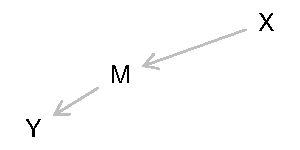
\includegraphics[height=0.5\textheight]{_nodes_and_claims_files/figure-beamer/unnamed-chunk-3-1} \end{center}

\begin{itemize}
\item
  ``Oil wealth produces grievances which cause conflict''
\item
  We often say: "\(M\) is a mechanism through which \(X\) causes \(Y\).
\end{itemize}
\end{frame}

\begin{frame}{Conditioning or moderating variables}
\protect\hypertarget{conditioning-or-moderating-variables}{}
\begin{center}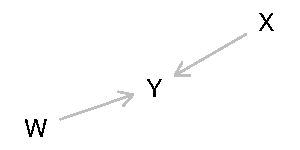
\includegraphics[height=0.5\textheight]{_nodes_and_claims_files/figure-beamer/unnamed-chunk-4-1} \end{center}

\begin{itemize}
\tightlist
\item
  e.g.~``The effect of oil wealth on conflict is weaker when
  institutions are strong''
\end{itemize}
\end{frame}

\begin{frame}{Variables might mediate \emph{and} moderate}
\protect\hypertarget{variables-might-mediate-and-moderate}{}
\begin{center}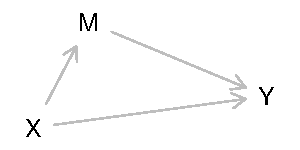
\includegraphics[height=0.5\textheight]{_nodes_and_claims_files/figure-beamer/unnamed-chunk-5-1} \end{center}

\begin{itemize}
\tightlist
\item
  ``Oil wealth produces grievances which cause conflict''\\
\item
  ``There are many other channels through which oil wealth affects
  conflict and which exacerbate the effects of grievances''
\end{itemize}
\end{frame}

\begin{frame}{Confounding variables}
\protect\hypertarget{confounding-variables}{}
\begin{center}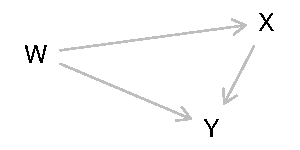
\includegraphics[height=0.5\textheight]{_nodes_and_claims_files/figure-beamer/unnamed-chunk-6-1} \end{center}

\begin{itemize}
\tightlist
\item
  ``The effect of education on voting behavior is hard to assess because
  wealth affects both education and voting behavior''
\end{itemize}
\end{frame}

\begin{frame}{Instrumental variables}
\protect\hypertarget{instrumental-variables}{}
\begin{center}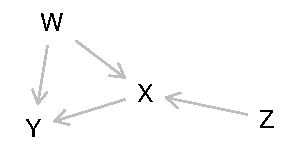
\includegraphics[height=0.5\textheight]{_nodes_and_claims_files/figure-beamer/unnamed-chunk-7-1} \end{center}

``It's hard to assess the effect of military service on future earnings
because of individual characteristics that might explain both. But date
of birth affects the chances of serving and so can be used to recover
estimates of service on earnings.''
\end{frame}

\end{document}
